\documentclass[14pt]{extarticle}
\def\activityid{F03-K-v3}\usepackage[letterpaper,margin=.65in,top=.60in,bottom=.65in]{geometry}
\usepackage{fix-cm}
\usepackage[T1]{fontenc}\usepackage[default]{sourcesanspro}
\usepackage{microtype,tikz,array,tabularx,fancyhdr,amsmath,amssymb}
\usepackage[hidelinks]{hyperref}\usetikzlibrary{calc,arrows.meta}
\setlength{\parindent}{0pt}\setlength{\parskip}{7pt}\setlength{\headheight}{0pt}\setlength{\footskip}{26pt}
\setlength{\emergencystretch}{2em}\pagestyle{fancy}\fancyhf{}\renewcommand{\headrulewidth}{0pt}\renewcommand{\footrulewidth}{.4pt}
\fancyfoot[L]{\scriptsize Bellingham Math Circle / Week 3 / \activityid}\fancyfoot[R]{\scriptsize \thepage}
\definecolor{ink}{gray}{.12}\definecolor{soft}{gray}{.95}\color{ink}
\newcommand{\PageTitle}[2]{{\fontsize{10}{12}\selectfont\bfseries WEEK 3\quad CODE MACHINES\hfill #1\par}\vspace{3pt}{\fontsize{26}{29}\selectfont\bfseries #2\par}\vspace{2pt}}
\newcommand{\NameLine}{{\small Name: \rule{2.65in}{.4pt}\hfill Date: \rule{1.35in}{.4pt}\par}\vspace{4pt}}
\newcommand{\Task}[2]{\par\vspace{3pt}{\large\bfseries #1}\par #2\par}
\newcommand{\Subhead}[1]{\par\vspace{3pt}{\large\bfseries #1}\par}
\newcommand{\RuleBox}[1]{\par\begingroup\setlength{\fboxsep}{8pt}\colorbox{soft}{\parbox{\dimexpr\linewidth-16pt\relax}{#1}}\endgroup\par}
\newcommand{\WriteBox}[2]{\par\textbf{#1}\par\vspace{2pt}\begin{tikzpicture}\draw[black!40,line width=.5pt] (0,0) rectangle (\dimexpr\linewidth-.5pt\relax,#2);\end{tikzpicture}\par}
\newcommand{\StudentFooter}{\vfill{\small Try it with objects. Explain by pointing, talking, or drawing.}\par}
\newcommand{\LampRing}[3]{\begin{tikzpicture}[x=1in,y=1in]
\foreach \i in {1,...,#1}{\coordinate (v\i) at ({90-360*(\i-1)/#1}:#2);}
\foreach \i in {1,...,#1}{\pgfmathtruncatemacro{\j}{mod(\i,#1)+1}\draw[thick] (v\i)--node[midway,fill=white,inner sep=2pt,font=\small]{\i\j}(v\j);}
\foreach \i in {1,...,#1}{\node[circle,draw,fill=white,minimum size=.52in,inner sep=0pt,font=\bfseries] at(v\i){\i};}
\foreach \i in {#3}{\node[circle,draw,fill=ink,text=white,minimum size=.52in,inner sep=0pt,font=\bfseries] at(v\i){\i};}
\end{tikzpicture}}
\newcommand{\Lights}[1]{\begin{tikzpicture}[x=.55in,y=.55in,baseline=-.10in]\foreach \v [count=\i] in {#1}{\ifnum\v=1\fill (\i,0) circle(.16in);\else\draw (\i,0) circle(.16in);\fi}\end{tikzpicture}}
\newcommand{\ClockRing}[2]{\begin{tikzpicture}[x=1in,y=1in]\draw[black!30] (0,0) circle(#2);\pgfmathtruncatemacro{\n}{#1-1}\foreach\i in {0,...,\n}{\node[circle,draw,fill=white,minimum size=.35in,inner sep=0pt] at({90-360*\i/#1}:#2){\i};}\draw[-{Stealth},thick] (-.35,.15) arc(155:25:.38);\node[font=\small] at(0,-.18){clockwise};\end{tikzpicture}}
\newcommand{\Key}[2]{\begin{center}\renewcommand{\arraystretch}{1.55}\begin{tabular}{c|*{#1}{c}}in&#2\end{tabular}\end{center}}


% v3 student pages use one running header and numbered tasks only.
\newcommand{\StudentHeader}[1]{{\fontsize{10}{12}\selectfont\bfseries Week 3 / Code machines / #1\par}\vspace{10pt}}
\newcommand{\Problem}[2]{\par\vspace{4pt}\textbf{Problem #1:} #2\par}
\newcommand{\Space}[1]{\begin{tikzpicture}\draw[black!35] (0,0) rectangle (\dimexpr\linewidth-.5pt\relax,#1);\end{tikzpicture}\par}
\newcommand{\Record}[2]{#1\par\Space{#2}}

\begin{document}
\StudentHeader{K--1}

\Problem{1}{One turn changes each symbol using this key. Keep its place in the message. Point to an input and follow its arrow. Try each symbol.}
\begin{center}{\LARGE\begin{tabular}{c@{\quad$\longrightarrow$\quad}c}$\bigcirc$&$\triangle$\\[9pt]$\triangle$&$\square$\\[9pt]$\square$&$\bigcirc$\end{tabular}}\end{center}
\Problem{2}{Send each message through the key. Draw or place its new symbols in the space beside it.}
\begin{center}\renewcommand{\arraystretch}{2.2}\begin{tabular}{c|p{3.6in}}Message&New message\\\hline$\bigcirc\ \triangle\ \bigcirc$&\\$\square\ \square\ \triangle$&\\$\triangle\ \bigcirc\ \square$&\\\end{tabular}\end{center}
\Problem{3}{A friend received triangle, circle, triangle. Follow the key backward to find the original message. Check by sending it forward again.}
\Space{.8in}

\newpage
\StudentHeader{K--1}

\Problem{4}{Use the same key. Start with a circle card. After every turn draw what it becomes. Keep going until the circle first comes back. Repeat from triangle and from square.}
\begin{center}\renewcommand{\arraystretch}{2.1}\begin{tabular}{c|p{.9in}|p{.9in}|p{.9in}}Start&Turn 1&Turn 2&Turn 3\\\hline$\bigcirc$&&&\\$\triangle$&&&\\$\square$&&&\\\end{tabular}\end{center}
\Problem{5}{These arrows show the same key as a loop. Move a counter one arrow each turn. Try all three starting shapes. Mark each arrival at its starting shape.}
\begin{center}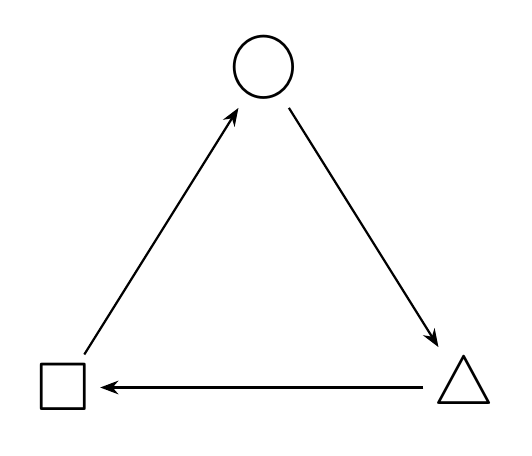
\begin{tikzpicture}[x=1in,y=1in,every node/.style={font=\Huge}]\node(A)at(0,1){$\bigcirc$};\node(B)at(1,-.6){$\triangle$};\node(C)at(-1,-.6){$\square$};\draw[-{Stealth},thick](A)--(B);\draw[-{Stealth},thick](B)--(C);\draw[-{Stealth},thick](C)--(A);\end{tikzpicture}\end{center}
\Problem{6}{Start with circle, triangle, square in a row. Change all three each turn. Stop when the whole row is back. Draw the row just before it comes back.}
\Space{.65in}

\newpage
\StudentHeader{K--1}

\Problem{7}{Change the key: circle and triangle swap; square stays square. Try all three starting shapes. Draw their results for two turns.}
\begin{center}{\Large$\bigcirc\leftrightarrow\triangle\qquad\square\longrightarrow\square$}\end{center}
\begin{center}\renewcommand{\arraystretch}{2.1}\begin{tabular}{c|p{1.6in}|p{1.6in}}Start&Turn 1&Turn 2\\\hline$\bigcirc$&&\\$\triangle$&&\\$\square$&&\\\end{tabular}\end{center}
\Problem{8}{Start with all three shapes in a row. Repeat this new key until the whole row returns. Compare with the old key. Record the number of turns for each.}
\Space{.85in}
\Problem{9}{Try another key: circle becomes square, and triangle also becomes square. Secretly choose circle or triangle and show only its output. Can your partner tell which input you chose? Swap roles and try again. Draw the two possible inputs.}
\Space{1in}

\end{document}
